%**************************************%
%*    Generated from PreTeXt source   *%
%*    on 2017-11-08T15:08:04-05:00    *%
%*                                    *%
%*   http://mathbook.pugetsound.edu   *%
%*                                    *%
%**************************************%
\documentclass[10pt,]{article}
%% Custom Preamble Entries, early (use latex.preamble.early)
%% Inline math delimiters, \(, \), need to be robust
%% 2016-01-31:  latexrelease.sty  supersedes  fixltx2e.sty
%% If  latexrelease.sty  exists, bugfix is in kernel
%% If not, bugfix is in  fixltx2e.sty
%% See:  https://tug.org/TUGboat/tb36-3/tb114ltnews22.pdf
%% and read "Fewer fragile commands" in distribution's  latexchanges.pdf
\IfFileExists{latexrelease.sty}{}{\usepackage{fixltx2e}}
%% Text height identically 9 inches, text width varies on point size
%% See Bringhurst 2.1.1 on measure for recommendations
%% 75 characters per line (count spaces, punctuation) is target
%% which is the upper limit of Bringhurst's recommendations
%% Load geometry package to allow page margin adjustments
\usepackage{geometry}
\geometry{letterpaper,total={340pt,9.0in}}
%% Custom Page Layout Adjustments (use latex.geometry)
%% This LaTeX file may be compiled with pdflatex, xelatex, or lualatex
%% The following provides engine-specific capabilities
%% Generally, xelatex and lualatex will do better languages other than US English
%% You can pick from the conditional if you will only ever use one engine
\usepackage{ifthen}
\usepackage{ifxetex,ifluatex}
\ifthenelse{\boolean{xetex} \or \boolean{luatex}}{%
%% begin: xelatex and lualatex-specific configuration
%% fontspec package will make Latin Modern (lmodern) the default font
\ifxetex\usepackage{xltxtra}\fi
\usepackage{fontspec}
%% realscripts is the only part of xltxtra relevant to lualatex 
\ifluatex\usepackage{realscripts}\fi
%% 
%% Extensive support for other languages
\usepackage{polyglossia}
%% Main document language is US English
\setdefaultlanguage{english}
%% Spanish
\setotherlanguage{spanish}
%% Vietnamese
\setotherlanguage{vietnamese}
%% end: xelatex and lualatex-specific configuration
}{%
%% begin: pdflatex-specific configuration
%% translate common Unicode to their LaTeX equivalents
%% Also, fontenc with T1 makes CM-Super the default font
%% (\input{ix-utf8enc.dfu} from the "inputenx" package is possible addition (broken?)
\usepackage[T1]{fontenc}
\usepackage[utf8]{inputenc}
%% end: pdflatex-specific configuration
}
%% Symbols, align environment, bracket-matrix
\usepackage{amsmath}
\usepackage{amssymb}
%% allow page breaks within display mathematics anywhere
%% level 4 is maximally permissive
%% this is exactly the opposite of AMSmath package philosophy
%% there are per-display, and per-equation options to control this
%% split, aligned, gathered, and alignedat are not affected
\allowdisplaybreaks[4]
%% allow more columns to a matrix
%% can make this even bigger by overriding with  latex.preamble.late  processing option
\setcounter{MaxMatrixCols}{30}
%%
%% Color support, xcolor package
%% Always loaded.  Used for:
%% mdframed boxes, add/delete text, author tools
\PassOptionsToPackage{usenames,dvipsnames,svgnames,table}{xcolor}
\usepackage{xcolor}
%%
%% Semantic Macros
%% To preserve meaning in a LaTeX file
%% Only defined here if required in this document
%% Subdivision Numbering, Chapters, Sections, Subsections, etc
%% Subdivision numbers may be turned off at some level ("depth")
%% A section *always* has depth 1, contrary to us counting from the document root
%% The latex default is 3.  If a larger number is present here, then
%% removing this command may make some cross-references ambiguous
%% The precursor variable $numbering-maxlevel is checked for consistency in the common XSL file
\setcounter{secnumdepth}{3}
%% Environments with amsthm package
%% Theorem-like environments in "plain" style, with or without proof
\usepackage{amsthm}
\theoremstyle{plain}
%% Numbering for Theorems, Conjectures, Examples, Figures, etc
%% Controlled by  numbering.theorems.level  processing parameter
%% Always need a theorem environment to set base numbering scheme
%% even if document has no theorems (but has other environments)
\newtheorem{theorem}{Theorem}[section]
%% Only variants actually used in document appear here
%% Style is like a theorem, and for statements without proofs
%% Numbering: all theorem-like numbered consecutively
%% i.e. Corollary 4.3 follows Theorem 4.2
\newtheorem{proposition}[theorem]{Task}
%% Definition-like environments, normal text
%% Numbering is in sync with theorems, etc
\theoremstyle{definition}
\newtheorem{definition}[theorem]{Definition}
%% Localize LaTeX supplied names (possibly none)
\renewcommand*{\proofname}{Proof}
%% Equation Numbering
%% Controlled by  numbering.equations.level  processing parameter
\numberwithin{equation}{section}
%% For improved tables
\usepackage{array}
%% Some extra height on each row is desirable, especially with horizontal rules
%% Increment determined experimentally
\setlength{\extrarowheight}{0.2ex}
%% Define variable thickness horizontal rules, full and partial
%% Thicknesses are 0.03, 0.05, 0.08 in the  booktabs  package
\makeatletter
\newcommand{\hrulethin}  {\noalign{\hrule height 0.04em}}
\newcommand{\hrulemedium}{\noalign{\hrule height 0.07em}}
\newcommand{\hrulethick} {\noalign{\hrule height 0.11em}}
%% We preserve a copy of the \setlength package before other
%% packages (extpfeil) get a chance to load packages that redefine it
\let\oldsetlength\setlength
\newlength{\Oldarrayrulewidth}
\newcommand{\crulethin}[1]%
{\noalign{\global\oldsetlength{\Oldarrayrulewidth}{\arrayrulewidth}}%
\noalign{\global\oldsetlength{\arrayrulewidth}{0.04em}}\cline{#1}%
\noalign{\global\oldsetlength{\arrayrulewidth}{\Oldarrayrulewidth}}}%
\newcommand{\crulemedium}[1]%
{\noalign{\global\oldsetlength{\Oldarrayrulewidth}{\arrayrulewidth}}%
\noalign{\global\oldsetlength{\arrayrulewidth}{0.07em}}\cline{#1}%
\noalign{\global\oldsetlength{\arrayrulewidth}{\Oldarrayrulewidth}}}
\newcommand{\crulethick}[1]%
{\noalign{\global\oldsetlength{\Oldarrayrulewidth}{\arrayrulewidth}}%
\noalign{\global\oldsetlength{\arrayrulewidth}{0.11em}}\cline{#1}%
\noalign{\global\oldsetlength{\arrayrulewidth}{\Oldarrayrulewidth}}}
%% Single letter column specifiers defined via array package
\newcolumntype{A}{!{\vrule width 0.04em}}
\newcolumntype{B}{!{\vrule width 0.07em}}
\newcolumntype{C}{!{\vrule width 0.11em}}
\makeatother
%% Figures, Tables, Listings, Named Lists, Floats
%% The [H]ere option of the float package fixes floats in-place,
%% in deference to web usage, where floats are totally irrelevant
%% You can remove some of this setup, to restore standard LaTeX behavior
%% HOWEVER, numbering of figures/tables AND theorems/examples/remarks, etc
%% may de-synchronize with the numbering in the HTML version
%% You can remove the "placement={H}" option to allow flotation and
%% preserve numbering, BUT the numbering may then appear "out-of-order"
%% Floating environments: http://tex.stackexchange.com/questions/95631/
\usepackage{float}
\usepackage{newfloat}
\usepackage[bf]{caption}
%% Adjust figure environment so that it no longer floats
\SetupFloatingEnvironment{figure}{fileext=lof,placement={H},within=section,name=Figure}
%% http://tex.stackexchange.com/questions/16195
\makeatletter
\let\c@figure\c@theorem
\makeatother
%% Adjust table environment so that it no longer floats
\SetupFloatingEnvironment{table}{fileext=lot,placement={H},within=section,name=Table}
%% http://tex.stackexchange.com/questions/16195
\makeatletter
\let\c@table\c@theorem
\makeatother
%% Raster graphics inclusion, wrapped figures in paragraphs
%% \resizebox sometimes used for images in side-by-side layout
\usepackage{graphicx}
%%
%% More flexible list management, esp. for references and exercises
%% But also for specifying labels (i.e. custom order) on nested lists
\usepackage{enumitem}
%% hyperref driver does not need to be specified, it will be detected
\usepackage{hyperref}
%% configure hyperref's  \url  to match listings' inline verbatim
\renewcommand\UrlFont{\small\ttfamily}
%% Hyperlinking active in PDFs, all links solid and blue
\hypersetup{colorlinks=true,linkcolor=blue,citecolor=blue,filecolor=blue,urlcolor=blue}
\hypersetup{pdftitle={Precalculus}}
%% If you manually remove hyperref, leave in this next command
\providecommand\phantomsection{}
%% Graphics Preamble Entries
\usepackage{tikz}  
\usepackage{pgfplots}
%% If tikz has been loaded, replace ampersand with \amp macro
\ifdefined\tikzset
    \tikzset{ampersand replacement = \amp}
\fi
%% extpfeil package for certain extensible arrows,
%% as also provided by MathJax extension of the same name
%% NB: this package loads mtools, which loads calc, which redefines
%%     \setlength, so it can be removed if it seems to be in the 
%%     way and your math does not use:
%%     
%%     \xtwoheadrightarrow, \xtwoheadleftarrow, \xmapsto, \xlongequal, \xtofrom
%%     
%%     we have had to be extra careful with variable thickness
%%     lines in tables, and so also load this package late
\usepackage{extpfeil}
%% Custom Preamble Entries, late (use latex.preamble.late)
%% Begin: Author-provided packages
%% (From  docinfo/latex-preamble/package  elements)
%% End: Author-provided packages
%% Begin: Author-provided macros
%% (From  docinfo/macros  element)
%% Plus three from MBX for XML characters

\newcommand{\lt}{<}
\newcommand{\gt}{>}
\newcommand{\amp}{&}
%% End: Author-provided macros
%% Title page information for article
\title{Precalculus}
\date{}
\begin{document}
%% Target for xref to top-level element is document start
\hypertarget{index}{}
\maketitle
\thispagestyle{empty}
\typeout{************************************************}
\typeout{Section 1 Learning Goals}
\typeout{************************************************}
\section[{Learning Goals}]{Learning Goals}\label{section-clg}
\hypertarget{p-1}{}%
In this section we give a list of learning goals for this notes. At the beginning of each section starting from Section 2, you will see a list of learning goals that will be addressed in that particular section.%
\leavevmode%
\begin{description}
\item[{1L}]\hypertarget{li-1}{}\hypertarget{p-2}{}%
Be able to solve a linear equation.%
\item[{2L}]\hypertarget{li-2}{}\hypertarget{p-3}{}%
Be able to determine the slope and the equation of a linear function given its graph or a table of values.%
\item[{3L}]\hypertarget{li-3}{}\hypertarget{p-4}{}%
Be able to model a situation with appropriate linear functions and interpret the solution.%
\item[{4Q}]\hypertarget{li-4}{}\hypertarget{p-5}{}%
Be able to solve a quadratic equation.%
\item[{5Q}]\hypertarget{li-5}{}\hypertarget{p-6}{}%
Be able to determine the vertex and the equation of a quadratic function given its graph or a table of values.%
\item[{6Q}]\hypertarget{li-6}{}\hypertarget{p-7}{}%
Be able to model a situation with appropriate quadratic functions and interpret the solution including interpreting the vertex in context.%
\item[{7E}]\hypertarget{li-7}{}\hypertarget{p-8}{}%
Be able to solve an equation that has an unknown exponent.%
\item[{8E}]\hypertarget{li-8}{}\hypertarget{p-9}{}%
Be able to determine the equation of a function of exponential type given its graph or a table of values.%
\item[{9E}]\hypertarget{li-9}{}\hypertarget{p-10}{}%
Be able to model a situation with appropriate functions of exponential type and interpret the solution.%
\item[{10E}]\hypertarget{li-10}{}\hypertarget{p-11}{}%
Be able to solve an equation that has logarithmic expressions.%
\item[{11E}]\hypertarget{li-11}{}\hypertarget{p-12}{}%
Be able to use the definitions and properties of exponential and logarithmic functions to rewrite or simplify algebraic expressions.%
\item[{12E}]\hypertarget{li-12}{}\hypertarget{p-13}{}%
Be able to use the definitions and properties of exponential and logarithmic functions to change their bases.%
\item[{13F}]\hypertarget{li-13}{}\hypertarget{p-14}{}%
Be able to determine inputs and outputs of a function from its graph and/or a table of values.%
\item[{14F}]\hypertarget{li-14}{}\hypertarget{p-15}{}%
Be able to determine the domain and range of function given as an equation or a graph.%
\item[{15F}]\hypertarget{li-15}{}\hypertarget{p-16}{}%
Be able to perform arithmetic (sum, difference, product, quotient) on functions given in any form (graph, table, equation).%
\item[{16F}]\hypertarget{li-16}{}\hypertarget{p-17}{}%
Be able to determine a composition of functions given in any form. (graph, table, equation).%
\item[{17F}]\hypertarget{li-17}{}\hypertarget{p-18}{}%
Be able to determine the inverse of a function given in any form (graph, table, equation).%
\item[{18F}]\hypertarget{li-18}{}\hypertarget{p-19}{}%
Be able to compute the average rate of change of a given function on a given interval.%
\item[{19F}]\hypertarget{li-19}{}\hypertarget{p-20}{}%
Be able to produce a graph of a given rational function and indicating the vertical and the horizontal asymptotes.%
\item[{20F}]\hypertarget{li-20}{}\hypertarget{p-21}{}%
Be able to solve inequalities and interpret the solution.%
\item[{21F}]\hypertarget{li-21}{}\hypertarget{p-22}{}%
Be able to identify the intervals on which a given function is increasing or decreasing.%
\item[{22F}]\hypertarget{li-22}{}\hypertarget{p-23}{}%
Be able to determine an appropriate function class (linear, quadratic, exponential, trigonometric) to model a particular situation.%
\item[{23F}]\hypertarget{li-23}{}\hypertarget{p-24}{}%
Be able to determine and describe a transformation (translations, compressions, stretches, reflections) of a function given in forms of graphs or equations.%
\item[{24T}]\hypertarget{li-24}{}\hypertarget{p-25}{}%
Be able to convert degrees and radians.%
\item[{25T}]\hypertarget{li-25}{}\hypertarget{p-26}{}%
Be able to determine the length of an arc of a circle or the area of a sector of a circle.%
\item[{26T}]\hypertarget{li-26}{}\hypertarget{p-27}{}%
Be able to use the distance formula or the equation of a circle in context.%
\item[{27T}]\hypertarget{li-27}{}\hypertarget{p-28}{}%
Be able to determine an angle or its trigonometric values given other trigonometric values and the quadrant.%
\item[{28T}]\hypertarget{li-28}{}\hypertarget{p-29}{}%
Be able to determine the equation of a trigonometric function given its graph.%
\item[{29T}]\hypertarget{li-29}{}\hypertarget{p-30}{}%
Be able to simplify functions using triangles that involve trigonometric and anti-trigonometric functions.%
\item[{30T}]\hypertarget{li-30}{}\hypertarget{p-31}{}%
Be able to prove trigonometric identities.%
\end{description}
\typeout{************************************************}
\typeout{Section 2 Linear Functions and Their Modeling}
\typeout{************************************************}
\section[{Linear Functions and Their Modeling}]{Linear Functions and Their Modeling}\label{section-linear}
\hypertarget{p-32}{}%
In this section, we address the following course learning goals.%
\leavevmode%
\begin{description}
\item[{1L}]\hypertarget{li-31}{}\hypertarget{p-33}{}%
Be able to solve a linear equation.%
\item[{2L}]\hypertarget{li-32}{}\hypertarget{p-34}{}%
Be able to determine the slope and the equation of a linear function given its graph or a table of values.%
\item[{3L}]\hypertarget{li-33}{}\hypertarget{p-35}{}%
Be able to model a situation with appropriate linear functions and interpret the solution.%
\item[{13F}]\hypertarget{li-34}{}\hypertarget{p-36}{}%
Be able to determine inputs and outputs of a function from its graph and/or a table of values.%
\item[{20F}]\hypertarget{li-35}{}\hypertarget{p-37}{}%
Be able to solve inequalities and interpret the solution.%
\end{description}
\begin{proposition}[{}]\label{motivation-linear}
\(2\)\(3\)\(4\)\(5\)\(1\)\leavevmode%
\begin{enumerate}
\item\hypertarget{li-36}{}Draw a picture that describes a \(2\) by \(2\) square pond, clearly indicating the portion of the pond and the portion of the tiles. How many tiles are needed to cover the border for this \(2\) by \(2\) square pond?%
\item\hypertarget{li-37}{}Repeat the last question for different pond sizes, from \(3\) by \(3\) up through \(6\) by \(6\). Make a table showing the number of border tiles needed for each size.%
\item\hypertarget{li-38}{}Based on the table that you created in the last part, if the side length of the pond is increased by \(1\) foot, how many more border tiles are needed? Explain why the number of tiles is increasing according to this pattern.%
\item\hypertarget{li-39}{}How many border tiles are needed for a pond with sides of length \(12\) feet?%
\item\hypertarget{li-40}{}If Nancy orders \(64\) border tiles for an upcoming job, how large is the pond the customer wants?%
\item\hypertarget{li-41}{}Write an equation for the number of tiles as a function of the length of one edge of the pond.%
\end{enumerate}
\end{proposition}
\hypertarget{p-38}{}%
The function that gives the number of tiles as a function of the length of one edge of the pond in the last problem is called a linear function. A \emph{linear function} is of the form%
\begin{equation*}
y=mx+b
\end{equation*}
where \(m\) is called the slope and \(b\) is the \(y\)-intercept of the function. If \((x_1,y_1), (x_2,y_2)\) are two different points on a linear function with \(x_1 \neq x_2\), then the slope of this linear function can be calculated using the formula%
\begin{equation*}
m = \frac{y_2-y_1}{x_2-x_1}
\end{equation*}
%
\begin{proposition}[{}]\label{proposition-2}
\leavevmode%
\begin{enumerate}
\item\hypertarget{li-42}{}Write an equation for the number of students as a function of years.%
\item\hypertarget{li-43}{}Below is a table that gives the number of students at Utica College from year 2012 to 2016. \leavevmode%
\begin{table}
\centering
\begin{tabular}{lc}\hrulemedium
Year&2012&2013&2014&2015&2016\tabularnewline\hrulemedium
Number of students&3718&3839&4028&4249&4463\tabularnewline\hrulemedium
\end{tabular}
\caption{Number of students at Utica College between 2012 and 2016\label{table-1}}
\end{table}
 Go to the link \href{https://www.desmos.com/calculator/bx2ueljf7x}{https://www.desmos.com/calculator/bx2ueljf7x} for a scatterplot of the data in the above table. Graph your function from the last question in the same coordinate system. How well is your function predicting the number of students at Utica College between 2012 and 2016?%
\item\hypertarget{li-44}{}According to this model, how many students are there in year 2017 at Utica College?%
\item\hypertarget{li-45}{}After what year will the number of students at Utica College be at least \(10,000\)?%
\end{enumerate}
\end{proposition}
\begin{proposition}[{}]\label{proposition-3}
\(2016\)\(9,315\)\(231\)\(2,547\)\(2016\)\(845\)\leavevmode%
\begin{enumerate}
\item\hypertarget{li-46}{}Write a function equation to estimate the total number of homes that are sold by Coldwell Banker as a function of the year \(t\).%
\item\hypertarget{li-47}{}Write a function equation to estimate the total number of homes that are sold by Assist2Sell as a function of the year \(t\).%
\item\hypertarget{li-48}{}Sketch the graph of both models in the same coordinate system using Desmos. When will the number of homes 	sold by these two real estate agencies equal?%
\item\hypertarget{li-49}{}When will the number of homes sold by Assit2Sell be double the number of homes sold by Coldwell Banker?%
\item\hypertarget{li-50}{}After what year will the number of homes sold by Assist2Sell be at least \(3,000\) more than the number of homes sold by Coldwell Banker?%
\end{enumerate}
\end{proposition}
\begin{proposition}[{}]\label{proposition-4}
\(F\)\(C\)\leavevmode%
\begin{enumerate}
\item\hypertarget{li-51}{}When traveling abroad, it can be useful to know the formula, but it is not necessary to remember the formula. One way to generate the formula is by remembering two temperatures on both scales. Why is it enough to remember just two temperatures in both scales?%
\item\hypertarget{li-52}{}Suppose we know that \(0^{\circ} C\) is \(32^{\circ} F\), and \(100^{\circ} C\) is \(212^{\circ} F\). Find the conversion formula that gives degree in Fahrenheit when we know degree in Celsius.%
\item\hypertarget{li-53}{}Find the conversion formula that gives degree in Celsius when we know degree in Fahrenheit.%
\item\hypertarget{li-54}{}Fill in the following table \leavevmode%
\begin{table}
\centering
\begin{tabular}{lc}\hrulemedium
Temp (degree in \(F\))&\(59\)&&\(77\)&\(86\)&\tabularnewline\hrulemedium
Temp (degree in \(C\))&&\(20\)&&&\(38\)\tabularnewline\hrulemedium
\end{tabular}
\caption{Temperature conversions\label{table-2}}
\end{table}
%
\item\hypertarget{li-55}{}At what temperature does it not matter to say Fehrenheit or Celsius?%
\end{enumerate}
\end{proposition}
\begin{proposition}[{}]\label{proposition-5}
\($1,099\)\(8.875\%\)\($20\)\leavevmode%
\begin{enumerate}
\item\hypertarget{li-56}{}Where should you buy the Apple laptop?%
\item\hypertarget{li-57}{}Now you want to create a model so that you know where to buy electronics in the future. First, create a function that calculates the final price \(P_1\) (in dollars) if the sales price of an electronics is \(x\) dollars assuming you are buying from the local Bestbuy store. (Final price includes tax.)%
\item\hypertarget{li-58}{}Now create a function  that calculates the final price \(P_2\) (in dollars) if the sales price of an electronics is \(x\) dollars assuming you are buying from Newegg.com. (Final price includes the flat shipping fee.)%
\item\hypertarget{li-59}{}Where should you buy electronics? Is one choice always better than the other choice? If so, which one is better? If not, how do you decide where to shop?%
\end{enumerate}
\end{proposition}
\typeout{************************************************}
\typeout{Section 3 Quadratic Functions and their modeling}
\typeout{************************************************}
\section[{Quadratic Functions and their modeling}]{Quadratic Functions and their modeling}\label{section-3}
\hypertarget{p-39}{}%
In this section, we address the following course learning goals.%
\leavevmode%
\begin{description}
\item[{4Q}]\hypertarget{li-60}{}\hypertarget{p-40}{}%
Be able to solve a quadratic equation.%
\item[{5Q}]\hypertarget{li-61}{}\hypertarget{p-41}{}%
Be able to determine the vertex and the equation of a quadratic function given its graph or a table of values.%
\item[{6Q}]\hypertarget{li-62}{}\hypertarget{p-42}{}%
Be able to model a situation with appropriate quadratic functions and interpret the solution including interpreting the vertex in context.%
\item[{13F}]\hypertarget{li-63}{}\hypertarget{p-43}{}%
Be able to determine inputs and outputs of a function from its graph and/or a table of values.%
\item[{14F}]\hypertarget{li-64}{}\hypertarget{p-44}{}%
Be able to determine the domain and range of function given as an equation or a graph.%
\item[{18F}]\hypertarget{li-65}{}\hypertarget{p-45}{}%
Be able to compute the average rate of change of a given function on a given interval.%
\item[{20F}]\hypertarget{li-66}{}\hypertarget{p-46}{}%
Be able to solve inequalities and interpret the solution.%
\item[{21F}]\hypertarget{li-67}{}\hypertarget{p-47}{}%
Be able to identify the intervals on which a given function is increasing or decreasing.%
\end{description}
\begin{proposition}[{}]\label{motivation-quadratic}
\(180\)\leavevmode%
\begin{enumerate}
\item\hypertarget{li-68}{}Pick your favorite length and width for the rectangular region so that twice the sum of length and width is equal to \(180\). Then calculate the area of the region.%
\item\hypertarget{li-69}{}Pick your second favorite length and width and repeat the process of the last question. Which dimension gives larger area?%
\item\hypertarget{li-70}{}Draw a diagram showing the rectangular area, and labeling the length of the region using a variable \(x\). Then find the width of the region in terms of the length\(x\). (Hint: You have \(180\) feet of wall materials.)%
\item\hypertarget{li-71}{}Write a function equation describing the area of the rectangular area \(A\) in terms of \(x\). Use Desmos to graph this function.%
\item\hypertarget{li-72}{}Using the graph of this function, decide how should the wall be built to get the maximum possible area. What is the maximum possible area?%
\end{enumerate}
\end{proposition}
\hypertarget{p-48}{}%
The function that gives the area of the rectangular region in terms of one side of the region is called a quadratic equation. In general, a \emph{quadratic equation} is a function of the form%
\begin{equation*}
f(x) = ax^2+bx+c
\end{equation*}
where \(a \neq 0\). We call this the \emph{general form} of a quadratic equation. Now try to rewrite the equation that you used in \hyperref[motivation-quadratic]{Task~1} in the form of \(f(x)=ax^2+bx+c\). What are the values of \(a, b\) and \(c\)?%
\par
\hypertarget{p-49}{}%
If we want to find the function equation of a quadratic equation give its graph, we have to pick three different points to plug in into the formula \(f(x)=ax^2+bx+c\) because we have to figure out the values of three unknowns \(a,b\) and \(c\). The computations will be lengthy because it involves solving a system of linear equations of three variables (it can be done pretty easily if you know how to use a computer package). We will not be doing this in this course. Instead, we will manipulate the function equation \(f(x)=ax^2+bx+c\) into a much desired form called the vertex form because a great deal of qualitative information about the function and its graph can simply be read off from this form. We will included the derivation in the following proof. Feel free to read the proof but it is not required.%
\begin{proof}\hypertarget{proof-1}{}
\hypertarget{p-50}{}%
Before we start doing the algebra, let us recall that%
\begin{equation*}
(X+Y)^2=X^2+2XY+Y^2.
\end{equation*}
We will need this formula from \hyperref[quadratic-step1]{(\ref{quadratic-step1})} to \hyperref[quadratic-step2]{(\ref{quadratic-step2})}.Now we manipulate the quadratic into a desired form.%
\begin{align}
f(x) \amp = ax^2+bx+c\label{mrow-1}\\
f(x) \amp = ax^2+bx+\frac{b^2}{4a} - \frac{b^2}{4a}+c\label{mrow-2}\\
f(x) \amp = a(x^2+\frac{b}{a}x+\frac{b^2}{4a^2}) - \frac{b^2}{4a}+c\label{mrow-3}\\
f(x) \amp = a(x^2+2\frac{b}{2a}x + (\frac{b}{2a})^2) - \frac{b^2}{4a}+c\label{quadratic-step1}\\
f(x) \amp = a(x+\frac{b}{2a})^2-\frac{b^2}{4a}+c\label{quadratic-step2}\\
f(x) \amp = a(x+\frac{b}{2a})^2-\frac{b^2-4ac}{4a}\label{quadratic-goodform}
\end{align}
By renaming \(h = -\frac{b}{2a}, k = -\frac{b^2-4ac}{4a},\) we have \(f(x)=a(x-h)^2+k\)%
\par
\hypertarget{p-51}{}%
Take Equation \hyperref[quadratic-goodform]{(\ref{quadratic-goodform})}, if we want to solve the quadratic equation%
\begin{equation*}
ax^2+bx+c = 0\text{,}
\end{equation*}
it is enough to solve the equation%
\begin{equation*}
a(x+\frac{b}{2a})^2-\frac{b^2-4ac}{4a} = 0
\end{equation*}
This is easy to solve because we have%
\begin{align}
a(x+\frac{b}{2a})^2-\frac{b^2-4ac}{4a} \amp = 0\label{mrow-7}\\
a(x+\frac{b}{2a})^2 \amp = \frac{b^2-4ac}{4a}\label{mrow-8}\\
(x+\frac{b}{2a})^2 \amp = \frac{b^2-4ac}{4a^2}\label{mrow-9}\\
x+\frac{b}{2a} \amp = \pm \sqrt{\frac{b^2-4ac}{4a^2}}\label{mrow-10}\\
x \amp = -\frac{b}{2a} \pm \sqrt{\frac{b^2-4ac}{4a^2}} \label{mrow-11}\\
x \amp = \frac{-b\pm\sqrt{b^2-4ac}}{2a}\label{quadratic-formula}
\end{align}
Equation \hyperref[quadratic-formula]{(\ref{quadratic-formula})} is the well-known quadratic formula that you have seen before.%
\end{proof}
\hypertarget{p-52}{}%
The \emph{vertex form} of a quadratic equation is of the form%
\begin{equation*}
f(x)=a(x-h)^2+k\text{.}
\end{equation*}
The reason this is called the vertex form is because we can read off the vertex of the graph, which is \((h,k)\). The \emph{vertex} of a quadratic function is the lowest point (if \(a \gt 0\)) or the highest point (if \(a \lt 0\)). Using the vertex form of a quadratic equation, we can find the function equation of a quadratic equation by first identifying the vertex (so we will know the values of \(h\) and \(k\)), and then pick a point on the graph of the quadratic equation other than the vertex to find the value of \(a\).%
\begin{proposition}[{}]\label{proposition-7}
\(k(x)\)\hyperref[quadratic-findformula]{Figure~3}\begin{figure}
\centering
\includegraphics[width=1\linewidth]{https://s3.amazonaws.com/grapher/exports/1diyeb1c8s.png}
\caption{Graph of \(k(x)\)\label{quadratic-findformula}}
\end{figure}
\leavevmode%
\begin{enumerate}
\item\hypertarget{li-73}{}What are the coordinates of the vertex of \(k(x)\)?%
\item\hypertarget{li-74}{}Write a function equation for \(k(x)\). Graph \(k(x)\) in Desmos.%
\item\hypertarget{li-75}{}Solve the quadratic equation \(k(x)=15\)%
\item\hypertarget{li-76}{}Solve the inequality \(k(x) \leq 15\).%
\item\hypertarget{li-77}{}Is it possible that \(k(x) = -11\)? What about \(200\)? What are the possible outputs of the function \(k(x)\)?%
\end{enumerate}
\end{proposition}
\begin{definition}[{}]\label{definition-1}
\emph{domain}\emph{range}\end{definition}
\begin{definition}[{}]\label{definition-2}
\(y=f(x)\)\emph{increasing}\(f(x)\)\(f(x)\)\emph{decreasing}\end{definition}
\begin{proposition}[{}]\label{proposition-8}
\(q(x)\)\hyperref[quadratic-findformulaagain]{Figure~7}\begin{figure}
\centering
\includegraphics[width=1\linewidth]{https://s3.amazonaws.com/grapher/exports/tqo3o3cjmv.png}
\caption{Graph of \(q(x)\)\label{quadratic-findformulaagain}}
\end{figure}
\leavevmode%
\begin{enumerate}
\item\hypertarget{li-78}{}Find \(q(-2)\).%
\item\hypertarget{li-79}{}What are the coordinates of the vertex of \(q(x)\)?%
\item\hypertarget{li-80}{}Write a function equation for \(q(x)\). Graph \(k(x)\) in Desmos.%
\item\hypertarget{li-81}{}Solve the quadratic equation \(q(x)=-6\)%
\item\hypertarget{li-82}{}Solve the inequality \(q(x) \leq -6\).%
\item\hypertarget{li-83}{}Solve the inequality \(q(x) \gt 2x-12\).%
\item\hypertarget{li-84}{}What is the domain and the range of the function \(q(x)\)?%
\item\hypertarget{li-85}{}On which interval is the function \(q(x)\) increasing? On which interval is the function \(q(x)\) decreasing?%
\end{enumerate}
\end{proposition}
\begin{definition}[{}]\label{definition-3}
\emph{average rate of change}\(f(x)\)\(a \le x \le b\)%
\begin{equation*}
\frac{f(b)-f(a)}{b-a}.
\end{equation*}
\end{definition}
\hypertarget{p-53}{}%
Note that the average rate of change computes the slope of the line between the two points \((a,f(a))\) and \((b,f(b))\).%
\begin{proposition}[{}]\label{proposition-9}
\(h(t) = -16t^2+vt+c\)\(t\)\(h(t)\)\(c\)\(v\)\leavevmode%
\begin{enumerate}
\item\hypertarget{li-86}{}If the pot falls, what is its initial velocity?%
\item\hypertarget{li-87}{}Suppose its takes \(3\) seconds for the pot to hit the ground. How high was the balcony?%
\item\hypertarget{li-88}{}Write down the function equation \(h(t)\) that gives the height of the flower pot at time \(t\).%
\item\hypertarget{li-89}{}What is the domain and the range of the function \(h(t)\)?%
\item\hypertarget{li-90}{}When is the flower pot at the height of \(100\) feet?%
\item\hypertarget{li-91}{}What is the average velocity of the flower pot from \(0\) second to \(3\) seconds?%
\end{enumerate}
\end{proposition}
\begin{proposition}[{}]\label{proposition-10}
\($90\)\(3,000\)\($5\)\(200\)\leavevmode%
\begin{enumerate}
\item\hypertarget{li-92}{}Make a table showing the price of concrete (per cubic yard), the amount of concrete sold per day, and the total income per day, for the prices of \($90\) to \($120\) per cubic yard, in \($5\) increments.%
\item\hypertarget{li-93}{}Write a function equation for the amount of concrete sold per day \(A\) as a function of the price of concrete \(p\).%
\item\hypertarget{li-94}{}Write an equation describing the total income for one day \(I(p)\) in terms of the price of concrete \(p\) .%
\item\hypertarget{li-95}{}What is the domain and the range of the function \(I(p)\)?%
\item\hypertarget{li-96}{}Suppose Mike will be satisfied if the total income for one day is at least \($268,000\). What are the possible price range (per cubic yard) he can charge to earn this income?%
\item\hypertarget{li-97}{}What price will Mike earn the maximum income per day? How many cubic yards of concrete will be sold per day? What is the maximum daily income?%
\end{enumerate}
\end{proposition}
\typeout{************************************************}
\typeout{Section 4 Exponential Functions and Their Modeling}
\typeout{************************************************}
\section[{Exponential Functions and Their Modeling}]{Exponential Functions and Their Modeling}\label{section-exp}
\hypertarget{p-54}{}%
In this section, we address the following course learning goals.%
\leavevmode%
\begin{description}
\item[{7E}]\hypertarget{li-98}{}\hypertarget{p-55}{}%
Be able to solve an equation that has an unknown exponent.%
\item[{8E}]\hypertarget{li-99}{}\hypertarget{p-56}{}%
Be able to determine the equation of a function of exponential type given its graph or a table of values.%
\item[{9E}]\hypertarget{li-100}{}\hypertarget{p-57}{}%
Be able to model a situation with appropriate functions of exponential type and interpret the solution.%
\item[{13F}]\hypertarget{li-101}{}\hypertarget{p-58}{}%
Be able to determine inputs and outputs of a function from its graph and/or a table of values.%
\item[{14F}]\hypertarget{li-102}{}\hypertarget{p-59}{}%
Be able to determine the domain and range of function given as an equation or a graph.%
\item[{15F}]\hypertarget{li-103}{}\hypertarget{p-60}{}%
Be able to perform arithmetic (sum, difference, product, quotient) on functions given in any form (graph, table, equation).%
\item[{18F}]\hypertarget{li-104}{}\hypertarget{p-61}{}%
Be able to compute the average rate of change of a given function on a given interval.%
\item[{20F}]\hypertarget{li-105}{}\hypertarget{p-62}{}%
Be able to solve inequalities and interpret the solution.%
\end{description}
\begin{proposition}[{}]\label{proposition-11}
\hypertarget{p-63}{}%
If we start with a single yeast cell under favorable growth conditions, then it will divide in one hour to form two identical "daughter cells". In turn, after another hour, each of these daughter cells will divide to produce two identical cells; we now have four identical "granddaughter cells" of the original parent cell. Under ideal conditions, this "doubling effect" will continue.%
\leavevmode%
\begin{enumerate}
\item\hypertarget{li-106}{}Create a table that contains the number of yeast cells \(N(t)\) at any given hours between \(t=0\) and \(t=8\).%
\item\hypertarget{li-107}{}How many yeast cells are there when \(t=100\)? (If you are stuck with this question or it takes too long, move on to the next question and then come back to this one later.)%
\item\hypertarget{li-108}{}Write a function equation of the number of yeast cells \(N(t)\) in terms of the hours \(t\).%
\item\hypertarget{li-109}{}If you were not able to answer Question 2, can you answer that question now using the function equation from Question 3?%
\end{enumerate}
\end{proposition}
\hypertarget{p-64}{}%
The function that models the number of yeast cells in terms of time is called an exponential function. In general, an \emph{exponential function} is a function of the form \(f(x)=b^x\) where \(b\gt0\). Here \(b\) is called the base and \(x\) is called the exponent. Let us first explore some properties of exponentials.%
\begin{proposition}[{}]\label{proposition-12}
\hypertarget{p-65}{}%
Consider three expressions that involve exponential functions \(2^x \times 3^y\), \((2 \times 3)^{xy}\), \((2 \times 3)^{x+y}\). By plugging in pairs of values for \(x\) and \(y\), decied whether any of these three expressions are the same or not.%
\end{proposition}
\begin{proposition}[{}]\label{proposition-13}
\hypertarget{p-66}{}%
Consider three expressions that involve exponential functions \(2^x \times 2^y\), \(2^{xy}\), \(2^{x+y}\). By plugging in pairs of values for \(x\) and \(y\), decied whether any of these three expressions are the same or not.%
\end{proposition}
\begin{proposition}[{}]\label{proposition-14}
\hypertarget{p-67}{}%
Consider three expressions that involve exponential functions \(2^x \times 3^x\), \((2 \times 3)^{x}\), \((2 + 3)^{x+x}\). By plugging in pairs of values for \(x\), decide whether any of these three expressions are the same or not.%
\end{proposition}
\begin{proposition}[{}]\label{proposition-15}
\hypertarget{p-68}{}%
Consider three expressions that involve exponential functions \((2^x)^y\), \(2^{x+y}\), \(2^{xy}\). By plugging in pairs of values for \(x\) and \(y\), decide whether any of these three expressions are the same or not.%
\end{proposition}
\hypertarget{p-69}{}%
Let us recall that for any \(b \gt 0\), we have \(b^0=1\), \(b^{-1} = \frac{1}{b}\). Let \(\frac{p}{q}\) be a rational number where \(q \gt 0\), we have%
\begin{equation*}
b^{\frac{p}{q}} = \sqrt[q]{b^p}.
\end{equation*}
%
\begin{proposition}[{}]\label{proposition-16}
\leavevmode%
\begin{enumerate}
\item\hypertarget{li-110}{}\(3^{-2}\)%
\item\hypertarget{li-111}{}\(8^{2/3}\)%
\item\hypertarget{li-112}{}\(4^{-3/2}\)%
\item\hypertarget{li-113}{}\(27^{-4/3}\)%
\end{enumerate}
\end{proposition}
\hypertarget{p-70}{}%
In application, exponential functions have a lot of limitations in many cases due to its simple nature. Instead, we use functions of exponential type. A function of exponential type is of the form \(f(x) = a \times b^x\) where \(a \neq 0\) and \(b \gt 0 \).%
\begin{proposition}[{}]\label{proposition-17}
\hypertarget{p-71}{}%
Let us re-consider the yeast cell growth problem. This time, we will start with three yeast cells instead of one.%
\leavevmode%
\begin{enumerate}
\item\hypertarget{li-114}{}Create a table that contains the number of yeast cells \(M(t)\) at any given hours between \(t=0\) and \(t=8\).%
\item\hypertarget{li-115}{}Can you use an exponential function to model this yeast cell growth problem?%
\item\hypertarget{li-116}{}Now model this problem using a function of exponential type. Write a function equation of the number of yeast cells \(M(t)\) in terms of the hours \(t\).%
\item\hypertarget{li-117}{}What is the domain and the range of the function \(M(t)\).%
\item\hypertarget{li-118}{}After how many hours will the number of yeast cells be exactly \(98304\)?%
\end{enumerate}
\end{proposition}
\begin{proposition}[{}]\label{proposition-18}
\hypertarget{p-72}{}%
Pam opens an investment account at Vanguard with \($10,000\). The account earns approximately \(6.5\%\) compounded annually. Let \(t\) be the number of years the account has been open, and \(B(t)\) the balance in the account.%
\leavevmode%
\begin{enumerate}
\item\hypertarget{li-119}{}Make a table showing the balance, \(B(t)\), in the account at \(t=0,1,2,3,\) and \(4\) years.%
\item\hypertarget{li-120}{}Write a function equation for the function \(B(t)\).%
\item\hypertarget{li-121}{}What is the domain and the range of the function \(B(t)\)?%
\item\hypertarget{li-122}{}Use your function equation to determine the balance in \(20\) years.%
\item\hypertarget{li-123}{}For the balance of the account to reach \($100,000\), at least how many years should Pam wait?%
\end{enumerate}
\end{proposition}
\begin{proposition}[{}]\label{proposition-19}
\hypertarget{p-73}{}%
The population of a small town has been growing. The population is shown in the following table.%
\begin{table}
\centering
\begin{tabular}{lc}\hrulemedium
\(t\) (years since 1980)&\(0\)&\(10\)&\(20\)&\(30\)\tabularnewline\hrulemedium
Population \(P(t)\)&\(2,354\)&\(3,164\)&\(4,252\)&\(5,714\)\tabularnewline\hrulemedium
\end{tabular}
\caption{Population of a small town\label{table-3}}
\end{table}
\leavevmode%
\begin{enumerate}
\item\hypertarget{li-124}{}What is the average number of people added to the town per year between 1980 and 2010?%
\item\hypertarget{li-125}{}Assuming that the population continues to grow exponentially, write a function equation for \(P(t)\).%
\item\hypertarget{li-126}{}If the population continues to grow according to the model, what is the population in 2015?%
\item\hypertarget{li-127}{}When will the population reach 10,000?%
\item\hypertarget{li-128}{}The gross domestic product (GDP) per capita of this small town in the year 1980 is \($83,145\) and has been increased at the rate of \(3.4\%\) every year since then. Write a function equation for the GDP per capita \(G(t)\) in terms of time \(t\) in years.%
\item\hypertarget{li-129}{}Write a function equation for the total GDP of this small town \(H(t)\) in terms of time \(t\) in years. Simplify the function equation as much as you can.%
\item\hypertarget{li-130}{}When will the total GDP of this small town reach one billion dollars?%
\item\hypertarget{li-131}{}Suppose that \(3\%\) of the annual GDP is spent on infrastructure. How much will be spent on infrastructure in this town in the year 2019?%
\end{enumerate}
\end{proposition}
\hypertarget{p-74}{}%
The Newton’s Law of Cooling (Warming) describes the principle of the heat loss of a body to its surroundings provided the temperature difference is small and the nature of radiating surface remains same. The temperature \(T\) of an object at time \(t\) is given by the formula%
\begin{equation*}
T(t)=T_a+(T_0 −T_a)e^{−kt}
\end{equation*}
where \(T(0) = T_0\) is the initial temperature of the object, \(T_a\) is the ambient temperature and \(k \gt 0\) is a constant that depends on the object. The letter \(e\) represents a number that is often used as the base in exponential functions because it has a number of special properties (you will learn more about this in calculus). The value of the number \(e\) is approximately \(2.718\).%
\begin{proposition}[{}]\label{proposition-20}
\hypertarget{p-75}{}%
A \(40^{\circ}\)F roast is cooked in a \(350^{\circ}\)F oven. After \(2\) hours, the temperature of the roast is \(125^{\circ}\)F.%
\leavevmode%
\begin{enumerate}
\item\hypertarget{li-132}{}Assuming the temperature of the roast follows Newton’s Law of Warming, find a formula for the temperature of the roast \(T(t)\) as a function of its time in the oven, \(t\), in hours.%
\item\hypertarget{li-133}{}The roast is done when the internal temperature reaches \(165^{\circ}\)F. When will the roast be done?%
\end{enumerate}
\end{proposition}
\typeout{************************************************}
\typeout{Section 5 Logarithmic Functions and Their Modeling}
\typeout{************************************************}
\section[{Logarithmic Functions and Their Modeling}]{Logarithmic Functions and Their Modeling}\label{section-log}
\hypertarget{p-76}{}%
In this section, we address the following course learning goals.%
\leavevmode%
\begin{description}
\item[{10E}]\hypertarget{li-134}{}\hypertarget{p-77}{}%
Be able to solve an equation that has logarithmic expressions.%
\item[{11E}]\hypertarget{li-135}{}\hypertarget{p-78}{}%
Be able to use the definitions and properties of exponential and logarithmic functions to rewrite or simplify algebraic expressions.%
\item[{12E}]\hypertarget{li-136}{}\hypertarget{p-79}{}%
Be able to use the definitions and properties of exponential and logarithmic functions to change their bases.%
\item[{14F}]\hypertarget{li-137}{}\hypertarget{p-80}{}%
Be able to determine the domain and range of function given as an equation or a graph.%
\item[{15F}]\hypertarget{li-138}{}\hypertarget{p-81}{}%
Be able to perform arithmetic (sum, difference, product, quotient) on functions given in any form (graph, table, equation).%
\item[{16F}]\hypertarget{li-139}{}\hypertarget{p-82}{}%
Be able to determine a composition of functions given in any form (graph, table, equation).%
\item[{17F}]\hypertarget{li-140}{}\hypertarget{p-83}{}%
Be able to determine the inverse of a function given in any form (graph, table, equation).%
\item[{22F}]\hypertarget{li-141}{}\hypertarget{p-84}{}%
Be able to determine an appropriate function class (linear, quadratic, exponential, trigonometric) to model a particular situation.%
\end{description}
\begin{proposition}[{}]\label{proposition-21}
\(n \times n\)\(4n+4\)\(1 \times 1\)\(1 \times 1\)\($30\)\(P(n)\)\(n\)\end{proposition}
\hypertarget{p-85}{}%
Given two functions \(y=f(x)\) and \(z=g(y)\), we can construct a new function \(z = (g \circ f)(x) = g(f(x))\), which is called the composition of \(g\) and \(f\).%
\begin{proposition}[{}]\label{proposition-22}
\(f(t)=t^2+1\)\(g(s) = 2s\)\leavevmode%
\begin{enumerate}
\item\hypertarget{li-142}{}Find the function equation of \((g \circ f)(x)\).%
\item\hypertarget{li-143}{}Find the function equation of \((f \circ g)(x)\).%
\item\hypertarget{li-144}{}Is \((g \circ f)(x)\) the same function as \((f \circ g)(x)\)? What does this tell you about the order of composition of two functions?%
\end{enumerate}
\end{proposition}
\begin{proposition}[{}]\label{proposition-23}
\(f(m)=2m+1\)\(g(p) = \frac{1}{2}p-\frac{1}{2}\)\leavevmode%
\begin{enumerate}
\item\hypertarget{li-145}{}Find the function equation of \((g \circ f)(x)\).%
\item\hypertarget{li-146}{}Find the function equation of \((f \circ g)(x)\).%
\item\hypertarget{li-147}{}Is \((g \circ f)(x)\) the same function as \((f \circ g)(x)\)?%
\end{enumerate}
\end{proposition}
\hypertarget{p-86}{}%
Given a function \(f\) defined on the domain \(D\) with the range \(E\) and another function \(g\) defined the domain \(E\) with the range \(D\). We say that \(g\) is the inverse function of \(f\) if \(g(f(x))=x\) for all \(x\) in \(D\) and \(f(g(x))=x\) for all \(x\) in \(E\). Often the inverse function \(g\) is denoted by \(f^{-1}\).%
\begin{proposition}[{}]\label{proposition-24}
\(z(t)=\sqrt{t-3}\)\leavevmode%
\begin{enumerate}
\item\hypertarget{li-148}{}What are the domain and the range of this function?%
\item\hypertarget{li-149}{}Find a function equation for the inverse function \(z^{-1}(t)\).%
\item\hypertarget{li-150}{}What are the domain and the range of \(z^{-1}\)?%
\end{enumerate}
\end{proposition}
\begin{proposition}[{}]\label{proposition-25}
\(h(x)=3x-7\)\leavevmode%
\begin{enumerate}
\item\hypertarget{li-151}{}What are the domain and the range of this function?%
\item\hypertarget{li-152}{}Find a function equation for the inverse function \(h^{-1}(t)\).%
\item\hypertarget{li-153}{}What are the domain and the range of \(h^{-1}\)?%
\end{enumerate}
\end{proposition}
\hypertarget{p-87}{}%
The inverse function of an exponential function \(f(x)=b^x\) is called the logarithmic function \(g(x)=\log_b(x)\). According to the definition of inverse functions, we know that \(f(g(x)) = x\) and \(g(f(x))=x\). Therefore we have%
\begin{equation*}
b^{\log_b(x)}=x, \qquad \log_b(b^x)=x.
\end{equation*}
This tells us that the number \(\log_b(x)\) is the exponent of \(b\) that gives \(x\), that is, if \(y=\log_b(x)\), then \(b^y=x\). When the base number \(b=e\), we write \(\log_b(x)\) as \(\ln(x)\) and call it the natural logarithmic function. We have%
\begin{equation*}
\ln(e^x) = x, \qquad e^{\ln(x)}=x. 
\end{equation*}
%
\begin{proposition}[{}]\label{proposition-26}
\leavevmode%
\begin{enumerate}
\item\hypertarget{li-154}{}What is the domain and the range of the function \(y=e^x\)?%
\item\hypertarget{li-155}{}What is the domain and the range of the function \(y=\ln(x)\)?%
\end{enumerate}
\end{proposition}
\begin{proposition}[{}]\label{proposition-27}
\leavevmode%
\begin{enumerate}
\item\hypertarget{li-156}{}\(\ln(\frac{1}{e})\).%
\item\hypertarget{li-157}{}\(e^{\ln(5)}\).%
\item\hypertarget{li-158}{}\(\frac{\ln(1)}{3}\).%
\item\hypertarget{li-159}{}\(2\ln(e)\).%
\end{enumerate}
\end{proposition}
\begin{proposition}[{}]\label{proposition-28}
\leavevmode%
\begin{enumerate}
\item\hypertarget{li-160}{}\(9 = 3^{x+1}\).%
\item\hypertarget{li-161}{}\((\frac{1}{2})^x=8\).%
\end{enumerate}
\end{proposition}
\begin{proposition}[{}]\label{proposition-29}
\(A, B\)\(r\)\leavevmode%
\begin{enumerate}
\item\hypertarget{li-162}{}For every positive numbers \(A, B\), \(\log_b(AB) = \log_b(A) + \log_b(B)\).%
\item\hypertarget{li-163}{}For every positive numbers \(A, B\), \(\log_b(A+B) = \log_b(A) + \log_b(B)\).%
\item\hypertarget{li-164}{}For every positive number \(A\) and every number \(r\), \(\log_b(A^r) = r\log_b(A)\).%
\item\hypertarget{li-165}{}For every positive numbers \(A, B\), \(\log_b(\frac{A}{B}) = \log_b(A) - \log_b(B)\).%
\item\hypertarget{li-166}{}For every positive numbers \(A, B\), \(\frac{\log_b(A)}{\log_b(B)} = \log_b(A) - \log_b(B)\).%
\item\hypertarget{li-167}{}For every positive numbers \(A, B\), \(\log_b(A - B) = \log_b(A) - \log_b(B)\).%
\end{enumerate}
\end{proposition}
\hypertarget{p-88}{}%
Note that \(\ln(x) = \log_e(x)\) so all the properties that hold for \(\log_b(x)\) for any base \(b\) also hold for \(\ln(x)\).%
\begin{proposition}[{}]\label{proposition-30}
\(\ln(2)\)\(\ln(3)\)\leavevmode%
\begin{enumerate}
\item\hypertarget{li-168}{}\(\ln(6)\).%
\item\hypertarget{li-169}{}\(\ln(\frac{2}{27})\).%
\end{enumerate}
\end{proposition}
\begin{proposition}[{}]\label{proposition-31}
\leavevmode%
\begin{enumerate}
\item\hypertarget{li-170}{}\(\log_4 (5x^3y)\).%
\item\hypertarget{li-171}{}\(\ln(\frac{\sqrt{3x-5}}{7})\).%
\end{enumerate}
\end{proposition}
\begin{proposition}[{}]\label{proposition-32}
\leavevmode%
\begin{enumerate}
\item\hypertarget{li-172}{}\(\frac{1}{2}\log_3(x)+3\log_3(x+1)\).%
\item\hypertarget{li-173}{}\(2\ln(x+2)-\ln(x)\).%
\end{enumerate}
\end{proposition}
\begin{proposition}[{}]\label{proposition-33}
\leavevmode%
\begin{enumerate}
\item\hypertarget{li-174}{}\(5+2\ln(x)=4\).%
\item\hypertarget{li-175}{}\(2\log_5(3x)=4\).%
\end{enumerate}
\end{proposition}
\hypertarget{p-89}{}%
On the Richter scale, the magnitude \(R\) of an earthquake of intensity \(I\) is given by%
\begin{equation*}
R = \log_{10} \frac{I}{I_0}.
\end{equation*}
Here \(I_0=1\) is the minimum intensity that can be detected and is used for comparison. Intensity is a measure of the wave energy of an earthquake.%
\begin{proposition}[{}]\label{proposition-34}
\leavevmode%
\begin{enumerate}
\item\hypertarget{li-176}{}North Bay, CA in August 24, 2014, \(R=6.0\) (Fatality: 1).%
\item\hypertarget{li-177}{}China in May 12, 2008, \(R=8.0\) (Fatalities: 87587).%
\end{enumerate}
\end{proposition}
\hypertarget{p-90}{}%
Common calculators can only calculate logarithm with base \(10\) or base \(e\). What if we want to calculate logarithms that have bases different from \(10\) and \(e\)? We can use the following base changing formula:%
\begin{equation*}
\log_b(x) = \frac{\log_a(x)}{\log_a(b)}.
\end{equation*}
%
\begin{proposition}[{}]\label{proposition-35}
\leavevmode%
\begin{enumerate}
\item\hypertarget{li-178}{}Calculate the value of \(\log_4(25)\) using the base changing formula with the new base \(10\).%
\item\hypertarget{li-179}{}Calculate the value of \(\log_4(25)\) using the base changing formula with the new base \(e\).%
\item\hypertarget{li-180}{}Compare your answers of the previous questions.%
\end{enumerate}
\end{proposition}
\begin{proposition}[{}]\label{proposition-36}
%
\begin{equation*}
\log_a(b) \times \log_b(x) = \log_a(x).
\end{equation*}
\leavevmode%
\begin{enumerate}
\item\hypertarget{li-181}{}First, simplify the exponential \(a^{\log_a(x)}\).%
\item\hypertarget{li-182}{}Second, simplify the exponential \(a^{\log_a(b) \times \log_b(x)}\) by first simplifying \(a^{\log_a(b)}\).%
\item\hypertarget{li-183}{}What can you say about \(a^{\log_a(x)}\) and \(a^{\log_a(b) \times \log_b(x)}\)? What does that tell you about \(\log_a(x)\) and \(\log_a(b) \times \log_b(x)\).%
\end{enumerate}
\end{proposition}
\hypertarget{p-91}{}%
We have learn several categories of functions such as linear functions, quadratic functions, exponential functions, logarithm functions. When given a set of data, how do we decide which type of functions we choose to model the set of the data?%
\begin{proposition}[{}]\label{proposition-37}
\href{https://www.desmos.com/calculator/lwopk4scwd}{https://www.desmos.com/calculator/lwopk4scwd}\end{proposition}
\typeout{************************************************}
\typeout{Section 6 Function Transformations and Rational Functions}
\typeout{************************************************}
\section[{Function Transformations and Rational Functions}]{Function Transformations and Rational Functions}\label{section-misc}
\hypertarget{p-92}{}%
In this section, we address the following course learning goals.%
\leavevmode%
\begin{description}
\item[{18F}]\hypertarget{li-184}{}\hypertarget{p-93}{}%
Be able to compute the average rate of change of a given function on a given interval.%
\item[{19F}]\hypertarget{li-185}{}\hypertarget{p-94}{}%
Be able to produce a graph of a given rational function and indicating the vertical and the horizontal asymptotes.%
\item[{20F}]\hypertarget{li-186}{}\hypertarget{p-95}{}%
Be able to solve inequalities and interpret the solution.%
\item[{21F}]\hypertarget{li-187}{}\hypertarget{p-96}{}%
Be able to identify the intervals on which a given function is increasing or decreasing.%
\item[{23F}]\hypertarget{li-188}{}\hypertarget{p-97}{}%
Be able to determine and describe a transformation (translations, compressions, stretches, reflections) of a function given in forms of graphs or equations.%
\end{description}
\hypertarget{p-98}{}%
In this section, we will examine how to build new functions from existing functions and how the graphs of the new functions relate to the original ones.%
\begin{proposition}[{}]\label{proposition-38}
\(f(x)=x^2\)\(h\)\(k\)\leavevmode%
\begin{enumerate}
\item\hypertarget{li-189}{}Write down the function formula for a new function \(g(x) = f(x-h)+k\).%
\item\hypertarget{li-190}{}Go to the link \href{https://www.desmos.com/calculator/z82wdytmxl}{https://www.desmos.com/calculator/z82wdytmxl}. Begin by setting \(h = 0\) and \(k=0\).%
\item\hypertarget{li-191}{}\hypertarget{p-99}{}%
The role of \(h\): %
\begin{enumerate}
\item\hypertarget{li-192}{}What happens as \(h\) increases from \(0\)?%
\item\hypertarget{li-193}{}What happens as \(h\) decreases from \(0\)?%
\item\hypertarget{li-194}{}Describes in words how different values of \(h\) affect the graph of the function \(g(x)\).%
\item\hypertarget{li-195}{}Without graphing, predict how the graph of \(q(x)=(x-4)^5\) will be different from the graph of \(p(x)=x^5\).%
\end{enumerate}
%
\item\hypertarget{li-196}{}\hypertarget{p-100}{}%
The role of \(k\): (Remember to reset \(h=0\) and \(k=0\)) %
\begin{enumerate}
\item\hypertarget{li-197}{}What happens as \(k\) increases from \(0\)?%
\item\hypertarget{li-198}{}What happens as \(k\) decreases from \(0\)?%
\item\hypertarget{li-199}{}Describes in words how different values of \(k\) affect the graph of the function \(g(x)\).%
\item\hypertarget{li-200}{}Without graphing, predict how the graph of \(q(x)=x^5-4\) will be different from the graph of \(p(x)=x^5\).%
\end{enumerate}
%
\end{enumerate}
\end{proposition}
\hypertarget{p-101}{}%
The role that \(h\) and \(k\) play can be summarized as horizontal and vertical shifts. Now we look at a different set of transformations.%
\begin{proposition}[{}]\label{proposition-39}
\(f(x)=e^x\)\leavevmode%
\begin{enumerate}
\item\hypertarget{li-201}{}Write down the function formula for two new functions \(g(x) = f(-x)\) and \(h(x) = -f(x)\).%
\item\hypertarget{li-202}{}Go to the link \href{https://www.desmos.com/calculator/r5bvx2qhjr}{https://www.desmos.com/calculator/r5bvx2qhjr}.Turn on the graphs of \(f(x)\) and \(g(x)\) in Desmos. How would you describe the procedure that obtains the graph of \(g(x)\) from the graph of \(f(x)\)?%
\item\hypertarget{li-203}{}Turn on the graphs of \(f(x)\) and \(h(x)\) in Desmos. How would you describe the procedure that obtains the graph of \(h(x)\) from the graph of \(f(x)\)?%
\end{enumerate}
\end{proposition}
\hypertarget{p-102}{}%
Shifts and reflections are called rigid transformations because the shape of the graph does not change. We now move to non-rigid transformations. But before that, we introduce a new function called the step function. The step function \(f(x) = \lfloor x \rfloor\) is defined to be the greatest integer less than or equal to \(x\). The step function is also called the floor function.%
\begin{proposition}[{}]\label{proposition-40}
\(\lfloor 1.5 \rfloor\)\(\lfloor -1.5 \rfloor\)\(\lfloor -10 \rfloor\)\end{proposition}
\begin{proposition}[{}]\label{proposition-41}
\(f(x)=\lfloor x \rfloor\)\(a\)\(b\)\leavevmode%
\begin{enumerate}
\item\hypertarget{li-204}{}Write down the function formula for a new function \(g(x) = af(bx)\).%
\item\hypertarget{li-205}{}Go to the link \href{https://www.desmos.com/calculator/qwuu0dswwf}{https://www.desmos.com/calculator/qwuu0dswwf}. Begin by setting \(a = 1\) and \(b = 1\).%
\item\hypertarget{li-206}{}\hypertarget{p-103}{}%
The role of \(a\): %
\begin{enumerate}
\item\hypertarget{li-207}{}What happens as \(a\) increases from \(1\)?%
\item\hypertarget{li-208}{}What happens as \(a\) decreases from \(1\) to \(0\)?%
\item\hypertarget{li-209}{}What happen when \(a = -1\)?%
\item\hypertarget{li-210}{}What happen as \(a\) increases from \(-1\) to \(0\)?%
\item\hypertarget{li-211}{}What happen as \(a\) decreases from \(-1\)?%
\item\hypertarget{li-212}{}Without graphing, predict how the graph of \(q(x)=-4x^5\) will be different from the graph of \(p(x)=x^5\).%
\end{enumerate}
%
\item\hypertarget{li-213}{}\hypertarget{p-104}{}%
The role of \(b\): (Remember to reset \(a=1\) and \(b=1\)) %
\begin{enumerate}
\item\hypertarget{li-214}{}What happens as \(b\) increases from \(1\)?%
\item\hypertarget{li-215}{}What happens as \(b\) decreases from \(1\) to \(0\)?%
\item\hypertarget{li-216}{}What happen when \(b = -1\)?%
\item\hypertarget{li-217}{}What happen as \(b\) increases from \(-1\) to \(0\)?%
\item\hypertarget{li-218}{}What happen as \(b\) decreases from \(-1\)?%
\item\hypertarget{li-219}{}Without graphing, predict how the graph of \(q(x)=(-4x)^5\) will be different from the graph of \(p(x)=x^5\).%
\end{enumerate}
%
\end{enumerate}
\end{proposition}
\begin{proposition}[{}]\label{proposition-42}
\(f(x)\)\(f(x)\)\(f(x)=x^2\)\leavevmode%
\begin{enumerate}
\item\hypertarget{li-220}{}\(3f(x-2)\)%
\item\hypertarget{li-221}{}\(f(3(x-2))\)%
\item\hypertarget{li-222}{}\(-3f(x+2)-5\)%
\item\hypertarget{li-223}{}\(3f(-3(x-2))-7\)%
\item\hypertarget{li-224}{}\(5f(3(x+2))+7\)%
\end{enumerate}
\end{proposition}
\hypertarget{p-105}{}%
A rational function is a quotient of polynomial functions that can be written as%
\begin{equation*}
f(x) = \frac{P(x)}{Q(x)}
\end{equation*}
where \(P(x), Q(x)\) are polynomials and \(Q(x)\) is not the zero polynomial. The domain of a rational function of \(x\) includes all real numbers except for a few \(x\)-values that make the denominator zero.%
\begin{proposition}[{}]\label{proposition-43}
\leavevmode%
\begin{enumerate}
\item\hypertarget{li-225}{}Find the domain and the range of \(f(x) = \frac{1}{x}\).%
\item\hypertarget{li-226}{}\hypertarget{p-106}{}%
Fill in the table \leavevmode%
\begin{table}
\centering
\begin{tabular}{lc}\hrulemedium
\(x\)&\(1\)&\(0.1\)&\(0.01\)&\(0.001\)\tabularnewline\hrulemedium
\(f(x)\)&\(\)&\(\)&\(\)&\(\)\tabularnewline\hrulemedium
\end{tabular}
\caption{Values of \(f(x)\) when \(x \to 0\)\label{table-4}}
\end{table}
 Create a similar table for \(x\) approaching to \(0\) from the negative side. Where do you think \(f(x)\) approaches to when \(x \to 0\)?%
\item\hypertarget{li-227}{}\hypertarget{p-107}{}%
Fill in the table \leavevmode%
\begin{table}
\centering
\begin{tabular}{lc}\hrulemedium
\(x\)&\(1\)&\(10\)&\(100\)&\(1000\)\tabularnewline\hrulemedium
\(f(x)\)&\(\)&\(\)&\(\)&\(\)\tabularnewline\hrulemedium
\end{tabular}
\caption{Values of \(f(x)\) when \(x \to +\infty\)\label{table-5}}
\end{table}
Where do you think \(f(x)\) approaches to when \(x \to +\infty\)? What about \(-\infty\)?%
\end{enumerate}
\end{proposition}
\begin{definition}[{}]\label{definition-4}
\(x=a\)\(f\)\(f(x) \to \infty\)\(f(x) \to -\infty\)\(x \to a\)\(y=b\)\(f\)\(f(x) \to b\)\(x \to +\infty\)\(x \to -\infty\)\end{definition}
\begin{proposition}[{}]\label{proposition-44}
\(f(x) = \frac{2x^2}{x^2-1}\)\leavevmode%
\begin{enumerate}
\item\hypertarget{li-228}{}Find the domain and the range of \(f(x)\).%
\item\hypertarget{li-229}{}Find all the vertical and horizontal asymptotes of \(f(x)\).%
\item\hypertarget{li-230}{}Find the intervals that \(f(x)\) is increasing and the intervals that \(f(x)\) is decreasing.%
\item\hypertarget{li-231}{}What is the average rate of change for \(3 \lt x \lt 6\)?%
\item\hypertarget{li-232}{}Solve the inequality \(f(x) \gt 3\).%
\end{enumerate}
\end{proposition}
\begin{proposition}[{}]\label{proposition-45}
\(f(x) = \frac{x^2+x-2}{x^2-x-6}\)\leavevmode%
\begin{enumerate}
\item\hypertarget{li-233}{}Find the domain and the range of \(f(x)\).%
\item\hypertarget{li-234}{}Find all the vertical and horizontal asymptotes of \(f(x)\).%
\item\hypertarget{li-235}{}Find the intervals that \(f(x)\) is increasing and the intervals that \(f(x)\) is decreasing.%
\item\hypertarget{li-236}{}What is the average rate of change for \(4 \lt x \lt 8\)?%
\item\hypertarget{li-237}{}Solve the inequality \(f(x) \gt 6\).%
\end{enumerate}
\end{proposition}
\typeout{************************************************}
\typeout{Section 7 Trigonometric Functions: Basics}
\typeout{************************************************}
\section[{Trigonometric Functions: Basics}]{Trigonometric Functions: Basics}\label{section-trig}
\hypertarget{p-108}{}%
In this section, we address the following course learning goals.%
\leavevmode%
\begin{description}
\item[{24T}]\hypertarget{li-238}{}\hypertarget{p-109}{}%
Be able to convert degrees and radians.%
\item[{25T}]\hypertarget{li-239}{}\hypertarget{p-110}{}%
Be able to determine the length of an arc of a circle or the area of a sector of a circle.%
\item[{26T}]\hypertarget{li-240}{}\hypertarget{p-111}{}%
Be able to use the distance formula or the equation of a circle in context.%
\item[{27T}]\hypertarget{li-241}{}\hypertarget{p-112}{}%
Be able to determine an angle or its trigonometric values given other trigonometric values and the quadrant.%
\end{description}
\hypertarget{p-113}{}%
Recall that the circumference of a circle of radius \(r\) is \(2\pi r\), and the area is \(\pi r^2\).%
\begin{proposition}[{}]\label{proposition-46}
\href{https://www.desmos.com/calculator/quxkgvqegp}{https://www.desmos.com/calculator/quxkgvqegp}\((2,3)\)\((-3,-2)\)\leavevmode%
\begin{enumerate}
\item\hypertarget{li-242}{}First find the length of the red line segment. How does this length relate to the \(x\)-coordinates of the two points?%
\item\hypertarget{li-243}{}Second find the length of the blue line segment. How does this length relate to the \(y\)-coordinates of the two points?%
\item\hypertarget{li-244}{}Third find the distance of the two points, namely the length of the green line segment. How does the distance of the two points relate to the \(x\) and the \(y\)-coordinates of the two points?%
\end{enumerate}
\((x_1,y_1)\)\((x_2,y_2)\)\end{proposition}
\hypertarget{p-114}{}%
A circle is a collection of points in the plane that are at a given distance, called the radius, from a given point, called the center. If we denote the radius by \(r\) and the center by \((h,k)\), the set of points \((x,y)\) satisfies the formula%
\begin{equation*}
(x-h)^2+(y-k)^2=r^2.
\end{equation*}
%
\begin{proposition}[{}]\label{proposition-47}
\((-4,-8)\)\(y\)\leavevmode%
\begin{enumerate}
\item\hypertarget{li-245}{}Draw a diagram of the circle in the \(xy\)-plane.%
\item\hypertarget{li-246}{}Write the equation of the circle.%
\item\hypertarget{li-247}{}Find the circumference and area of the circle.%
\end{enumerate}
\end{proposition}
\begin{proposition}[{}]\label{proposition-48}
\((-6,-4)\)\((-1,8)\)\leavevmode%
\begin{enumerate}
\item\hypertarget{li-248}{}Draw a diagram of the circle in the \(xy\)-plane.%
\item\hypertarget{li-249}{}Write the equation of the circle.%
\item\hypertarget{li-250}{}Find the circumference and area of the circle.%
\end{enumerate}
\end{proposition}
\hypertarget{p-115}{}%
It is well-know that one of the way to measure angles is using degrees. One full rotation is \(360^{\circ}\), half of a rotation is \(180^{\circ}\) and a right angle is \(90^{\circ}\). We now introduce another unit to measure angles, called radian, that is based on the arc length cut by the angle, and the radius. Note that the circumference of the circle with radius \(1\) is equal to \(2\pi\) so we say that one full rotation is \(2\pi\) radian (or simply rad). Half of a rotation is \(\pi\) rad and a right is \(\frac{\pi}{2}\) rad.%
\begin{proposition}[{}]\label{proposition-49}
\(0^{\circ}, 30^{\circ}, 45^{\circ}, 60^{\circ}, 120^{\circ}, 135^{\circ}, 150^{\circ}\)\end{proposition}
\hypertarget{p-116}{}%
An arc of a circle is a piece of a circle, and has length. A sector is a part of the plane enclosed by two radii and an arc of a circle, and has area.%
\begin{proposition}[{}]\label{proposition-50}
\leavevmode%
\begin{enumerate}
\item\hypertarget{li-251}{}What is the length of the arc along a circle of radius \(7\) cut out by an angle of \(90^{\circ}\)?%
\item\hypertarget{li-252}{}What is the length of the arc along a circle of radius \(3\) cut out by an angle of \(45^{\circ}\)?%
\item\hypertarget{li-253}{}What is the length of the arc along a circle of radius \(5\) cut out by an angle of \(30^{\circ}\)?%
\item\hypertarget{li-254}{}\hypertarget{p-117}{}%
Fill in the following table \leavevmode%
\begin{table}
\centering
\begin{tabular}{cc}\hrulemedium
Angle measured in degree&Angle measured in radian&Radius&Arc length\tabularnewline\hrulemedium
\(90^{\circ}\)&\(\)&\(7\)&\(\)\tabularnewline\hrulemedium
\(45^{\circ}\)&\(\)&\(3\)&\(\)\tabularnewline\hrulemedium
\(30^{\circ}\)&\(\)&\(5\)&\(\)\tabularnewline\hrulemedium
\end{tabular}
\caption{Using radian to calculate arc length\label{table-6}}
\end{table}
 Then create a formula that calculates the length of an arc using the radian of the angle.%
\end{enumerate}
\end{proposition}
\begin{proposition}[{}]\label{proposition-51}
\leavevmode%
\begin{enumerate}
\item\hypertarget{li-255}{}What is the area of the sector cut out of a circle of radius \(7\) cut out by an angle of \(90^{\circ}\)?%
\item\hypertarget{li-256}{}What is the area of the sector cut out of a circle of radius \(3\) cut out by an angle of \(45^{\circ}\)?%
\item\hypertarget{li-257}{}What is the area of the sector cut out of a circle of radius \(5\) cut out by an angle of \(30^{\circ}\)?%
\item\hypertarget{li-258}{}\hypertarget{p-118}{}%
Fill in the following table \leavevmode%
\begin{table}
\centering
\begin{tabular}{cc}\hrulemedium
Angle measured in degree&Angle measured in radian&Radius&Sector area\tabularnewline\hrulemedium
\(90^{\circ}\)&\(\)&\(7\)&\(\)\tabularnewline\hrulemedium
\(45^{\circ}\)&\(\)&\(3\)&\(\)\tabularnewline\hrulemedium
\(30^{\circ}\)&\(\)&\(5\)&\(\)\tabularnewline\hrulemedium
\end{tabular}
\caption{Using radian to calculate sector area\label{table-7}}
\end{table}
 Then create a formula that calculates the area of a sector using the radian of the angle.%
\end{enumerate}
\end{proposition}
\hypertarget{p-119}{}%
From now on, we will be using radian to measure angles unless otherwise specified. We now discuss the six trigonometric functions of angles between \(0\) and \(\frac{\pi}{2}\) in the right triangles. After that we will discuss trigonometric functions for any angles.%
\begin{figure}
\centering
{
\begin{tikzpicture}
	\coordinate [label=left:$C$] (C) at (-1.5cm,-1.cm);
	\coordinate [label=right:$A$] (A) at (1.5cm,-1.0cm);
	\coordinate [label=above:$B$] (B) at (1.5cm,1.0cm);
	\draw (C) -- node[above] {hyp} (B) -- node[right] {opp} (A) -- node[below] {adj} (C);
	\coordinate [label=right:$\alpha$] (D) at (-1.3cm,-0.85cm);
\end{tikzpicture}
}
\caption{A right triangle\label{figure-3}}
\end{figure}
\hypertarget{p-120}{}%
Using the lengths of these three sides, you can form six ratios that define the six trigonometric functions of the angle \(\alpha\).%
\begin{equation*}
\text{sine, cosine, tangent, cotangent, secant, cosecant.}
\end{equation*}
Note that \(0 \lt \alpha \lt \frac{\pi}{2}\) and the definitions below do not work angles that are outside of this range. We use the following abbrevations: opp for the length of the side opposite to \(\alpha\), adj for the length of the side adjacent to \(\alpha\), hyp for the length of the hypotenuse.%
\begin{equation*}
\sin(\alpha) = \frac{\text{opp}}{\text{hyp}}, \qquad \cos(\alpha) = \frac{\text{adj}}{\text{hyp}}, \qquad \tan(\alpha) = \frac{\text{opp}}{\text{adj}}
\end{equation*}
%
\begin{equation*}
\csc(\alpha) = \frac{\text{hyp}}{\text{opp}}, \qquad \sec(\alpha) = \frac{\text{hyp}}{\text{adj}}, \qquad \cot(\alpha) = \frac{\text{adj}}{\text{opp}}
\end{equation*}
%
\begin{proposition}[{}]\label{proposition-52}
\(\Delta DEF\)\(E\)\(DF=4\)\(EF=2\)\(DE\)\(\sin(\angle EDF), \cos(\angle EDF), \tan(\angle EDF), \cot(\angle EDF), \sec(\angle EDF), \csc(\angle EDF)\)\end{proposition}
\begin{proposition}[{}]\label{problem-verifysimpletrigid}
\(\displaystyle \sin(\frac{\pi}{4}), \cos(\frac{\pi}{4}), \tan(\frac{\pi}{4}), \cot(\frac{\pi}{4}), \sec(\frac{\pi}{4}), \csc(\frac{\pi}{4})\)\leavevmode%
\begin{enumerate}
\item\hypertarget{li-259}{}\(\displaystyle \sin^2(\frac{\pi}{4}) + \cos^2(\frac{\pi}{4})\)%
\item\hypertarget{li-260}{}\(\displaystyle \sec^2(\frac{\pi}{4}) - \tan^2(\frac{\pi}{4})\)%
\item\hypertarget{li-261}{}\(\displaystyle \csc^2(\frac{\pi}{4}) - \cot^2(\frac{\pi}{4})\)%
\end{enumerate}
\end{proposition}
\begin{figure}
\centering
{
\begin{tikzpicture}
	\coordinate [label=left:$C$] (C) at (-1.5cm,-1.0cm);
	\coordinate [label=right:$A$] (A) at (1.5cm,-1.0cm);
	\coordinate [label=above:$B$] (B) at (1.5cm,2.0cm);
	\draw (C) -- (B) -- node[right] {$1$} (A) -- node[below] {$1$} (C);
	\coordinate [label=right:$\frac{\pi}{4}$] (D) at (-1.2cm,-0.75cm);
	\coordinate [label=below:$\frac{\pi}{4}$] (E) at (1.3cm,1.8cm);
\end{tikzpicture}
}
\caption{An isosceles triangle\label{figure-4}}
\end{figure}
\begin{proposition}[{}]\label{task-30-60}
\(\displaystyle \frac{\pi}{6}\)\(\displaystyle \frac{\pi}{3}\)\hyperref[problem-verifysimpletrigid]{Task~11}\(\displaystyle \frac{\pi}{6}\)\(\displaystyle \frac{\pi}{3}\)\(BD\)\end{proposition}
\begin{figure}
\centering
{
\begin{tikzpicture}
	\coordinate [label=left:$C$] (C) at (-1.5cm,-1.0cm);
	\coordinate [label=right:$A$] (A) at (1.5cm,-1.0cm);
	\coordinate [label=above:$B$] (B) at (0cm,1.6cm);
	\coordinate [label=below:$D$] (D) at (0cm,-1.0cm);
	\draw (C) -- node[below] {$1$} (D) -- node[below] {$1$} (A) -- node[right] {$2$} (B) -- node[left] {$2$} (C);
	\draw (B) -- (D);
	\coordinate [label=right:$\frac{\pi}{6}$] (E) at (-0.15cm,1.0cm);
	\coordinate [label=below:$\frac{\pi}{3}$] (F) at (1.1cm,-0.4cm);
\end{tikzpicture}
}
\caption{A \(30^{\circ}\)-\(60^{\circ}\)-\(90^{\circ}\) triangle\label{figure-5}}
\end{figure}
\begin{proposition}[{}]\label{proposition-55}
\(115\)\(78.3^{\circ}\)\end{proposition}
\begin{proposition}[{}]\label{proposition-56}
\hyperref[skatboard]{Figure~17}\(c\)\(b\)\end{proposition}
\begin{figure}
\centering
{
\begin{tikzpicture}
	\coordinate (C) at (-1.5cm,-1.cm);
	\coordinate (A) at (1.5cm,-1.0cm);
	\coordinate (B) at (1.5cm,1.0cm);
	\draw (C) -- node[above] {$c$} (B) -- node[right] {$b$} (A) -- node[below] {$13$ feet} (C);
	\coordinate [label=right:$18.4^{\circ}$] (D) at (-1.2cm,-0.85cm);
\end{tikzpicture}
}
\caption{A skateboard ramp.\label{skatboard}}
\end{figure}
\hypertarget{p-121}{}%
Now we know how to define trigonometric functions for angles between \(0\) and \(\frac{\pi}{2}\), what about angles larger than \(\frac{\pi}{2}\)? In order to do that, we need to use the unit circle.%
\begin{figure}
\centering
{
\begin{tikzpicture}
	\draw [thick] (0,0) circle (3cm);
	\draw [thick ->] (-3.5,0) -- (3.5,0) node[right] {$x$};
	\draw [thick ->] (0,-3.5) -- (0,3.5) node[right] {$y$};
	\draw (0,0) --  (1.5,2.6) node[above] {$(x,y)$};
	\draw (1.5,0) -- (1.5,2.6);
	\draw (0,0.2) -- (0,0.2) node[right] {$\alpha$};
\end{tikzpicture}
}
\caption{The Unit Circle\label{unit-circle}}
\end{figure}
\begin{proposition}[{}]\label{proposition-57}
\((x,y)\)\(\alpha\)\(x\)\((x,y)\)\(x\)\(y\)\(\alpha\)\(1\)\end{proposition}
\begin{proposition}[{}]\label{proposition-58}
\hyperref[unit-circle-fill-in]{Figure~21}\leavevmode%
\begin{enumerate}
\item\hypertarget{li-262}{}First fill in the box with the measure of angle in radian.%
\item\hypertarget{li-263}{}Second using the answers of \hyperref[problem-verifysimpletrigid]{Task~11} and \hyperref[task-30-60]{Task~13} to figure out the coordinate of the points of \(30^{\circ}, 45^{\circ}\) and \(60^{\circ}\).%
\item\hypertarget{li-264}{}Third using properties of symmetry to figure out the coordinate of the points of \(120^{\circ}, 135^{\circ}\) and \(150^{\circ}\).%
\item\hypertarget{li-265}{}Fourth using the same idea as in the last question to figure out the rest of the coordinates in the unit circle.%
\end{enumerate}
\end{proposition}
\begin{figure}
\centering
{
\begin{tikzpicture} [>=stealth, baseline=0,scale=2.5, angle/.style={draw,text=white,fill=white,minimum height=1cm, minimum width=1cm},point/.style={white}]


	\draw [white] (-3.6,-3.6) rectangle (3.6,3.6);
	\draw [thick,fill=white] (0,0) circle (3cm);
	\draw [thick, ->] (-3.3,0) -- (3.3,0);
	\draw [thick, ->] (0,-3.3) -- (0,3.3);
	\draw (0,0) --  node [angle] {$\frac{\pi}{2}$} (90:3) node[point, above right] {$ \left(0,1\right) $};
	\draw (0,0) --  node [angle] {\footnotesize{$\pi$}} (180:3) node[point, above left] {$ \left(-1,0\right) $};
	\draw (0,0) --  node [angle] {$\frac{3\pi}{2}$} (270:3) node[point, below right] {$ \left(0,-1\right) $};
	\draw (0,0) --  node [angle] {\footnotesize{$2\pi$}} (0:3) node[point, above right] {$ \left(1,0\right) $};
	\draw (0,0) --  node [angle] {$\frac{\pi}{4}$} (45:3)  node [point, above right] {$ \left( \frac{\sqrt2}{2} , \frac{\sqrt2}{2}  \right) $};
	\draw (0,0) --  node [angle] {$\frac{3\pi}{4}$} (135:3) node [point, above left] {$ \left( -\frac{\sqrt2}{2} , \frac{\sqrt2}{2}  \right) $};
	\draw (0,0) --  node [angle] {$\frac{5\pi}{4}$} (225:3) node [point, below left] {$ \left( -\frac{\sqrt2}{2} , -\frac{\sqrt2}{2}  \right) $};
	\draw (0,0) --  node [angle] {$\frac{7\pi}{4}$} (315:3) node [point, below right] {$ \left( \frac{\sqrt2}{2} , -\frac{\sqrt2}{2}  \right) $};
	\draw (0,0) --  node [near end, angle] {$\frac{\pi}{6}$} (30:3) node [point, above right] {$ \left( \frac{\sqrt3}{2} , \frac{1}{2}  \right) $};
	\draw (0,0) --  node [near end, angle] {$\frac{\pi}{3}$} (60:3) node [point, above right] {$ \left( \frac{1}{2} , \frac{\sqrt3}{2}  \right) $};
	\draw (0,0) --  node [near end, angle] {$\frac{2\pi}{3}$} (120:3) node [point, above left] {$ \left( -\frac{1}{2} , \frac{\sqrt3}{2}  \right) $};
	\draw (0,0) --  node [near end, angle] {$\frac{5\pi}{6}$} (150:3) node [point, above left] {$ \left(- \frac{\sqrt3}{2} , \frac{1}{2}  \right) $};
	\draw (0,0) --  node [near end, angle] {$\frac{7\pi}{6}$} (210:3) node [point, below left] {$ \left(- \frac{\sqrt3}{2} , -\frac{1}{2}  \right) $};
	\draw (0,0) --  node [near end, angle] {$\frac{4\pi}{3}$} (240:3) node [point, below left] {$ \left( -\frac{1}{2} , -\frac{\sqrt3}{2}  \right) $};
	\draw (0,0) --  node [near end, angle] {$\frac{5\pi}{3}$} (300:3) node [point, below right] {$ \left( \frac{1}{2} , -\frac{\sqrt3}{2}  \right) $};
	\draw (0,0) --  node [near end, angle] {$\frac{11\pi}{6}$} (330:3) node [point, below right] {$ \left( \frac{\sqrt3}{2} , -\frac{1}{2}  \right) $};

	\foreach \n in {1,2,3,4}
	\foreach \t in {0,30,45,60}
	\fill (\n*90+\t:3) circle (0.03cm);
	\foreach \t in {30,45,60, 120,135,150, 210,225,240, 300,315,330}
	\node [font=\tiny, fill=white,inner sep=1pt] at (\t:.75) {$ \t\degree $};
\end{tikzpicture}
}
\caption{The Unit Circle\label{unit-circle-fill-in}}
\end{figure}
\begin{proposition}[{}]\label{proposition-59}
\hyperref[unit-circle-fill-in]{Figure~21}\end{proposition}
\begin{table}
\centering
\begin{tabular}{c}\hrulemedium
&\(\sin\)&\(\cos\)&\(\tan\)&\(\cot\)&\(\sec\)&\(\csc\)\tabularnewline\hrulemedium
\(0^{\circ}\)&&&&&&\tabularnewline\hrulemedium
\(30^{\circ}\)&&&&&&\tabularnewline\hrulemedium
\(45^{\circ}\)&&&&&&\tabularnewline\hrulemedium
\(60^{\circ}\)&&&&&&\tabularnewline\hrulemedium
\(90^{\circ}\)&&&&&&\tabularnewline\hrulemedium
\(120^{\circ}\)&&&&&&\tabularnewline\hrulemedium
\(135^{\circ}\)&&&&&&\tabularnewline\hrulemedium
\(150^{\circ}\)&&&&&&\tabularnewline\hrulemedium
\(180^{\circ}\)&&&&&&\tabularnewline\hrulemedium
\(210^{\circ}\)&&&&&&\tabularnewline\hrulemedium
\(225^{\circ}\)&&&&&&\tabularnewline\hrulemedium
\(240^{\circ}\)&&&&&&\tabularnewline\hrulemedium
\(270^{\circ}\)&&&&&&\tabularnewline\hrulemedium
\(300^{\circ}\)&&&&&&\tabularnewline\hrulemedium
\(315^{\circ}\)&&&&&&\tabularnewline\hrulemedium
\(330^{\circ}\)&&&&&&\tabularnewline\hrulemedium
\end{tabular}
\caption{Trig values for important angles\label{table-8}}
\end{table}
\typeout{************************************************}
\typeout{Section 8 Trigonometric Functions: Additonal Topics}
\typeout{************************************************}
\section[{Trigonometric Functions: Additonal Topics}]{Trigonometric Functions: Additonal Topics}\label{section-trig-adv}
\hypertarget{p-122}{}%
In this section, we address the following course learning goals.%
\leavevmode%
\begin{description}
\item[{28T}]\hypertarget{li-266}{}\hypertarget{p-123}{}%
Be able to determine the equation of a trigonometric function given its graph.%
\item[{29T}]\hypertarget{li-267}{}\hypertarget{p-124}{}%
Be able to simplify functions using triangles that involve trigonometric and anti-trigonometric functions.%
\item[{30T}]\hypertarget{li-268}{}\hypertarget{p-125}{}%
Be able to prove trigonometric identities.%
\end{description}
\hypertarget{p-126}{}%
We start this section by investigating graphs of trigonometric functions. The following is the graph of \(y=\sin(x)\)%
\begin{figure}
\centering
{
\begin{tikzpicture}
\begin{axis}[width=13.5cm, height=5cm, axis x line=center, axis y line=middle, samples=100, ymin=-1.5, ymax=1.5, xmin=-7.0, xmax=7.0, domain=-2*pi:2*pi, xtick={-6.28318, -4.7123889, -3.14159, -1.5708, 1.5708, 3.14159, 4.7123889, 6.28318}, xticklabels={$-2\pi$, $-\frac{3\pi}{2}$, $-\pi$, $-\frac{\pi}{2}$, $\frac{\pi}{2}$, $\pi$, $\frac{3\pi}{2}$, $2\pi$}]
\addplot [] {sin(deg(x))};
\end{axis}
\end{tikzpicture}
}
\caption{The Graph of \(y=\sin(x)\)\label{graph-sin}}
\end{figure}
\hypertarget{p-127}{}%
Note that the maximum value of the sine curve can take is \(1\) and the minimum value is \(-1\). The range of the sine function is \([-1,1]\). The amplitude represents half the distance between the maximum and minimum values of the function and thus it is equal to \(1\).%
\begin{proposition}[{}]\label{proposition-60}
\(a\)%
\begin{equation*}
y=a\sin(b(x-h))+k
\end{equation*}
\href{https://www.desmos.com/calculator/qsvc9fflcg}{https://www.desmos.com/calculator/qsvc9fflcg}\leavevmode%
\begin{enumerate}
\item\hypertarget{li-269}{}What happens as \(a\) increases from \(1\)?%
\item\hypertarget{li-270}{}What happens as \(a\) decreases from \(1\) to \(0\)?%
\item\hypertarget{li-271}{}What is the relationship between \(a\) and the amplitude?%
\end{enumerate}
\end{proposition}
\hypertarget{p-128}{}%
The mid-line of the sine curve is the horizontal line that runs exactly in the middle of the maximum and the minimum of the curve. Thus the mid-line is \(y=0\).%
\begin{proposition}[{}]\label{proposition-61}
\(k\)%
\begin{equation*}
y=a\sin(b(x-h))+k
\end{equation*}
\href{https://www.desmos.com/calculator/qsvc9fflcg}{https://www.desmos.com/calculator/qsvc9fflcg}\leavevmode%
\begin{enumerate}
\item\hypertarget{li-272}{}What happens as \(k\) increases from \(0\)?%
\item\hypertarget{li-273}{}What happens as \(k\) decreases from \(0\)?%
\item\hypertarget{li-274}{}What is the relationship between \(k\) and the midline?%
\end{enumerate}
\end{proposition}
\hypertarget{p-129}{}%
The period is the horizontal length of one cycle of the sine curve (such as from one peak to the next peak). The period of the sine curve is \(2\pi\).%
\begin{proposition}[{}]\label{proposition-62}
\(b\)%
\begin{equation*}
y=a\sin(b(x-h))+k
\end{equation*}
\href{https://www.desmos.com/calculator/qsvc9fflcg}{https://www.desmos.com/calculator/qsvc9fflcg}\begin{table}
\centering
\begin{tabular}{cc}\hrulemedium
Values of \(b\)&Period\tabularnewline\hrulemedium
\(1\)&\(\)\tabularnewline\hrulemedium
\(4\)&\(\)\tabularnewline\hrulemedium
\(2\)&\(\)\tabularnewline\hrulemedium
\(2\pi\)&\(\)\tabularnewline\hrulemedium
\(\frac{\pi}{2}\)&\(\)\tabularnewline\hrulemedium
\(\frac{\pi}{4}\)&\(\)\tabularnewline\hrulemedium
\end{tabular}
\caption{Relations between period and \(b\)\label{table-9}}
\end{table}
\(b\)\(b\)\(b\)\(b\)\end{proposition}
\begin{proposition}[{}]\label{proposition-63}
\(h\)%
\begin{equation*}
y=a\sin(b(x-h))+k
\end{equation*}
\href{https://www.desmos.com/calculator/qsvc9fflcg}{https://www.desmos.com/calculator/qsvc9fflcg}\leavevmode%
\begin{enumerate}
\item\hypertarget{li-275}{}What happens as \(h\) increases from \(0\)?%
\item\hypertarget{li-276}{}What happens as \(k\) decreases from \(0\)?%
\end{enumerate}
\end{proposition}
\begin{proposition}[{}]\label{proposition-64}
\leavevmode%
\begin{enumerate}
\item\hypertarget{li-277}{}\(y=14\sin(2\pi x)+4\).%
\item\hypertarget{li-278}{}\(y=-\frac{1}{2}\sin(\frac{\pi}{2}(x-1))+\frac{2}{3}\).%
\end{enumerate}
\end{proposition}
\begin{proposition}[{}]\label{proposition-65}
%
\begin{equation*}
y=a\cos(b(x-h))+k.
\end{equation*}
\href{https://www.desmos.com/calculator/mka32cuaa8}{https://www.desmos.com/calculator/mka32cuaa8}\(a,b,h,k\)\end{proposition}
\begin{proposition}[{}]\label{proposition-66}
\leavevmode%
\begin{figure}
\centering
\IfFileExists{images/trig-graph-problem.pdf}%
{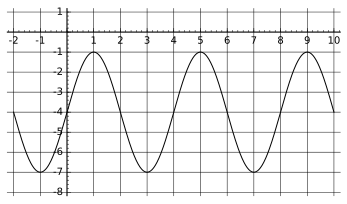
\includegraphics[width=1\linewidth]{images/trig-graph-problem.pdf}}%
{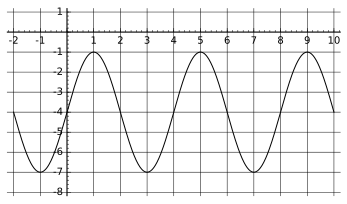
\includegraphics[width=1\linewidth]{images/trig-graph-problem.png}}
\caption{A graph of a trig function\label{figure-10}}
\end{figure}
\leavevmode%
\begin{enumerate}
\item\hypertarget{li-279}{}Write a function equation for the function of the form \(a\sin(b(x-h))+k\).%
\item\hypertarget{li-280}{}Write a function equation for the function of the form \(a\cos(b(x-h))+k\).%
\end{enumerate}
\end{proposition}
\hypertarget{p-130}{}%
We now move to discuss inverse trigonometric functions. We started with the inverse sine function.%
\begin{definition}[{}]\label{definition-5}
\(y=\arcsin(x)\)\(\sin(y)=x\)\(-1 \leq x \leq 1\)\(-\frac{\pi}{2} \leq y \leq \frac{\pi}{2}\)\(y=\arcsin(x)\)\([-1,1]\)\([-\frac{\pi}{2},\frac{\pi}{2}]\)\end{definition}
\hypertarget{p-131}{}%
The domain of the sine function is all real numbers and the range of the sine function is \([-1,1]\). Notice that the domain of the inverse sine function is \([-1,1]\) but the range is \([-\frac{\pi}{2},\frac{\pi}{2}]\), not all real numbers.%
\begin{proposition}[{}]\label{proposition-67}
\(\arcsin(-\frac{1}{2})\)\(\arcsin(\frac{\sqrt{3}}{2})\)\(\arcsin(-2)\)\end{proposition}
\begin{definition}[{}]\label{definition-6}
\(y=\arccos(x)\)\(\cos(y)=x\)\(-1 \leq x \leq 1\)\(0 \leq y \leq \pi\)\(y=\arccos(x)\)\([-1,1]\)\([0,\pi]\)\(y=\arctan(x)\)\(\tan(y)=x\)\(-\infty \leq x \leq \infty\)\(-\frac{\pi}{2} \leq y \leq \frac{\pi}{2}\)\(y=\arctan(x)\)\((-\infty,\infty)\)\([-\frac{\pi}{2},\frac{\pi}{2}]\)\end{definition}
\begin{proposition}[{}]\label{proposition-68}
\(\arccos(\frac{\sqrt{2}}{2})\)\(\arctan(0)\)\(\arctan(-1)\)\end{proposition}
\hypertarget{p-132}{}%
Recall that for any function \(f\) that has an inverse function \(f^{-1}\), we have \(f(f^{-1}(x))=x\) and \(f^{-1}(f(x))=x\). One caveat is that these formulas are only true if \(x\) is the correct domain.%
\begin{proposition}[{}]\label{proposition-69}
\leavevmode%
\begin{enumerate}
\item\hypertarget{li-281}{}\(\tan(\arctan(-5))\)%
\item\hypertarget{li-282}{}\(\arcsin(\sin(\frac{5\pi}{3}))\)%
\item\hypertarget{li-283}{}\(\cos(\arccos(\pi))\)%
\end{enumerate}
\end{proposition}
\hypertarget{p-133}{}%
Now we look at how to evaluate compositions of trigonometric functions and inverse trigonometric functions that are not of the same origins.%
\begin{proposition}[{}]\label{proposition-70}
\(\tan(\arccos\frac{2}{3})\)\leavevmode%
\begin{enumerate}
\item\hypertarget{li-284}{}First, let us call \(\arccos(\frac{2}{3})=\alpha\). Create a right triangle such that one of the non-right triangles is \(\alpha\) and \(\cos(\alpha)=\frac{2}{3}\).%
\item\hypertarget{li-285}{}Second, find out the value of \(\tan(\alpha)\).%
\item\hypertarget{li-286}{}Third, find out the value of \(\tan(\arccos\frac{2}{3})\).%
\end{enumerate}
\end{proposition}
\begin{proposition}[{}]\label{proposition-71}
\(\cos(\arcsin(-\frac{3}{5}))\)\end{proposition}
\hypertarget{p-134}{}%
Note that by the definition of the basic six trigonometric functions, we have \(\cot(x) = \frac{1}{\tan(x)}\), \(\sec(x) = \frac{1}{\cos(x)}\), and \(\csc(x) = \frac{1}{\sin(x)}\). These relationships between trigonometric functions are called trigonometric identities. Here "identities" stands for "equalities". Note that a trigonometric identity involves trigonometric functions of an arbitrary angle and not a specific angle. As a counterexample, \(\sin(\frac{\pi}{2}) = 1\) is not a trigonometric identity because it is about one specific angle \(\frac{\pi}{2}\). The big question is that are there any other identities. How do we find out?%
\begin{proposition}[{}]\label{proposition-72}
\leavevmode%
\begin{enumerate}
\item\hypertarget{li-287}{}Look at \hyperref[problem-verifysimpletrigid]{Task~\ref{problem-verifysimpletrigid}}. Can you find some trigonometric identities? If so, write down the trigonometric identities.%
\item\hypertarget{li-288}{}Now look at the trigonometric identities that you discovered in the last part, replace the trigonometric functions in the trigonometric identities with the definition of the trigonometric functions. (If you don't remember the definiton, go back to the last unit to review them.) Then try to justify that the trigonomtric identities are true. (This is called a proof!)%
\end{enumerate}
\end{proposition}
\hypertarget{p-135}{}%
In order to prove a trigonometric identity, we can use other trigonometric identities that have been established. The more identities that we have established, the larger our toolbox will be. When trying to prove a trigonometric identity, start working with the side that is more than complicated than the other. This allows you to manipulate the expression using algebra to get the simpler form.%
\begin{proposition}[{}]\label{proposition-73}
\hypertarget{p-136}{}%
Prove the identity%
\begin{equation*}
\tan(x)\csc(x) = \sec(x)\text{.}
\end{equation*}
%
\end{proposition}
\begin{proposition}[{}]\label{proposition-74}
\hypertarget{p-137}{}%
Prove the identity%
\begin{equation*}
\frac{\sec^2(\theta)-1}{\sec^2(\theta)} = \sin^2(\theta)\text{.}
\end{equation*}
%
\end{proposition}
\begin{proposition}[{}]\label{proposition-75}
\hypertarget{p-138}{}%
Prove the identity%
\begin{equation*}
\frac{\sin^2(\theta)+\cos^2(\theta)}{\cos^2(\theta)\sec^2(\theta)} = 1\text{.}
\end{equation*}
%
\end{proposition}
\begin{proposition}[{}]\label{proposition-76}
\hypertarget{p-139}{}%
Prove the identity%
\begin{equation*}
(\tan^2(x)+1)(\cos^2(x)-1)=-\tan^2(x)\text{.}
\end{equation*}
%
\end{proposition}
\begin{proposition}[{}]\label{proposition-77}
\hypertarget{p-140}{}%
Prove the identity%
\begin{equation*}
\tan(x)+\cot(x)=\sec(x)\csc(x)\text{.}
\end{equation*}
%
\end{proposition}
\begin{proposition}[{}]\label{proposition-78}
\hypertarget{p-141}{}%
Prove the identity%
\begin{equation*}
\frac{\cot^2(\theta)}{1+\csc(\theta)} = \frac{1 - \sin(\theta)}{\sin(\theta)}\text{.}
\end{equation*}
%
\end{proposition}
\end{document}